\documentclass[a4paper, 12pt]{article}
\usepackage{comment} % enables the use of multi-line comments (\ifx \fi) 
\usepackage{lipsum} %This package just generates Lorem Ipsum filler text. 
\usepackage{fullpage} % changes the margin
\usepackage[utf8]{inputenc}
\usepackage{algorithm}
\usepackage{algorithmicx}
\usepackage{algpseudocode}
\usepackage{graphicx}

\begin{document}
%Header-Make sure you update this information!!!!
\noindent
\large\textbf{Documentação TP2} \hfill \textbf{Ícaro Harry} \\
\normalsize AEDS3 \hfill  Matrícula: 2014033050\\


\section{Introdução}
\paragraph{}
O trabalho proposto no TP2 foi a resolução do Problema do Caixeiro Viajante, utilizando uma abordagem de "podas" (estratégias de \textit{branch and bound}). Para isso, são dadas restrições de precedência para a visitação de cidades, onde se existe uma restrição entre A e B, A deve ser visitada \textbf{antes} do que B. O problema, em sua versão de decisão, consiste em um clássico NP Completo. Ou seja, não existe solução em tempo polinomial  conhecida. Isso faz com que resolver instâncias relativamente pequenas do problema demande um poder de processamento inexistente na atualidade. 
\paragraph{}
A ideia das estratégias de \textit{branch and bound} consiste em limitar (podar) a árvore de possíveis soluções do problema, eliminando a necessidade de verificar certos caminhos. Dessa maneira, a solução que desenvolvi para o problema, executando podas, é capaz de executar determinadas instâncias do PCV em um tempo razoável.

\section{Modelagem do Problema}
\paragraph{}
O problema proposto é um clássico PCV (Problema do Caixeiro Viajante), onde todas as cidades possuem ligações entre si. A única diferença no enunciado é a existência de \textit{restrições de precedência}, as quais determinam que algumas cidades devem ser visitadas antes do que outras.

\subsection{Grafo de cidades}
\paragraph{}
Utilizei o método de \textbf{matriz de adjacências} para implementar os grafos.
\paragraph{}
As cidades são representadas por meio de um \textbf{grafo não-direcionado completo}, onde as arestas representam as distâncias entre as cidades. Esse grafo não é direcionado pois, pela descrição do problema, não existe diferença entre os caminhos de ida e volta entre duas cidades.


\subsection{Grafo de restrições}
\paragraph{}
As restrições são representadas por um \textbf{grafo direcionado sem peso}, onde uma aresta entre o vértice \textbf{A} e o vértice \textbf{B}, representa uma restrição de que \textbf{A} deve ser vistada antes do que \textbf{B}. Porém, existe a necessidade de que esse grafo seja direcionada, já que existe uma diferença entre uma restrição de A para B e de B para A.

\subsection{Caminhamento pelas cidades}
\paragraph{}
O Problema do Caixeiro Viajante consiste em percorrer \textbf{todos} os (n-1)! possíveis caminhos para verificar qual o menor deles. Dessa maneira, para percorrer todos esses caminhos, necessita-se de um algoritmo que permute todas as possíveis ordens de visita aos vértices. Para fazer isso, utilizei o algoritmo de \textit{DFS (Depth First Search, ou Busca em Profundidade)}, modificado. 
\paragraph{}
O algoritmo de busca em profundidade, em sua versão recursiva, percorre um caminho até o final e na volta, percorre os vértices adjacentes, recursivamente. Além disso, por meio de um vetor \textit{booleano}, o algoritmo verifica quais vértices já foram visitados, para não percorrê-los novamente. Todavia, para que todos os possíveis caminhos sejam visitados, é necessário que os vértices que foram marcados como visitados, sejam desmarcados, ao final da recursão, para que possam ser visitados novamente, dessa vez em outra ordem.

\begin{algorithm}
\caption{ModifiedDFS}
\begin{algorithmic}
\Function{DFS}{$G$, $v$, $n$, $visited$}
    \State $visited$[$v$] = true;
    \For{$i$ = 0; $i$ minor than $n$; $i$++}
		\If{!$visited$[$i$]}
			\State DFS($G$, $i$, $n$);
			\State $visited$[$i$] = false;			
		\EndIf  
    \EndFor
\EndFunction
\end{algorithmic}
\end{algorithm}




\subsection{Métodos de Branch and Bound (podas)}
\paragraph{}
Como dito anteriormente, para localizar o menor caminho, deve-se percorrer todas as possíveis combinações de vértices, o que torna o algoritmo fatorial (O(n!)). Dessa maneira, para o número máximo de cidades do problema (22), é necessário verificar 21! caminhos, o que demoraria anos para ser executado em um PC comum. Todavia, é possível reduzir a árvore de possíveis soluções, utilizando técnicas de \textit{podas}, onde, dada determinada configuração, é possível concluir que ela não levará ao resultado ótimo, e assim, é possível eliminá-la antes de checá-la até o final, evitando-se visitar diversos vértices. Sendo assim, descreverei todas as podas que realizei em minha solução.

\paragraph{}
É importante destacar que, além de podas que são "intrínsecas" ao PCV, as restrições de precedência propostas no enunciado, permitem podar ainda mais a árvore de possíveis soluções. Já que, ao encontrar uma aresta que desrespeita uma restrição, não é necessário continuar visitando os vértices após essa aresta.

\subsubsection{Poda do caminho atual - \textit{(Poda 1)}}
\paragraph{}
A poda mais simples realizada é a que verifica se o menor caminho já visitado é menor ou igual ao caminho que se está verificando atualmente. Se isso ocorrer, o caminho atual não é promissor, ou seja, é impossível que ele seja o menor de todos.
\paragraph{}
É simples realizar essa poda. Basta armazenar em uma variável o menor caminho já encontrado até agora e compará-lo ao caminho percorrido, caso a aresta até o próximo vértice a ser visitado, somada ao caminho atual, iguale ou ultrapasse o menor caminho atual, não se chama a recursão para aquele vértice.

\begin{algorithm}
\caption{ModifiedDFS with the first branch and bound}
\begin{algorithmic}
\Function{DFS}{$G$, $v$, $n$, $visited$, $current$, $minimum$}
    \State $visited$[$v$] = true;
    \For{$i$ = 0; $i$ minor than $n$; $i$++}
		\If{!$visited$[$i$]}
			\If{($current$ + $G$[$v$][$i$] minor than $minimum$)}
				\State DFS($G$, $i$, $n$);
				\State $visited$[$i$] = false;			
			\EndIf
		\EndIf
    \EndFor
\EndFunction
\end{algorithmic}
\end{algorithm}

\subsubsection{Poda do caminho da volta - \textit{(Poda 2)}}
\paragraph{}
Outra poda que pode ser realizada é a poda de eliminar o caminho da volta. Como o grafo não é direcionado, temos que a aresta de A para B é igual a aresta de B para A. Dessa maneira, ao permutar todos os possíveis caminhos, o caminho da ida e o caminho da volta vão ser verificados, mas na prática, eles representam o mesmo caminho. Por exemplo, dada as cidades A, B, C, D e E o caminho ABCDEA é igual ao caminho AEDCBA. Entretando, quando existe uma restrição de B para C, todos os caminhos em que C aparece antes de B, podem ser descartados, o que reduz pela metada a árvore de caminhos. Como mostrado nos exemplos:

\paragraph{}
\textbf{Caminhos onde B aparece depois de C: } CBDE, CBED, CDBE, CDEB, CEBD, CEDB, DCBE, DCEB, DECB, ECBD, ECDB, EDCB.

\paragraph{}
\textbf{Caminhos onde B aparece antes de C: } BCDE, BCED, BDCE, BDEC, BEDC, BECD, DBEC, DBCE, DEBC, EBCD, EBDC, EDBC.

\paragraph{}
Portanto, se não existe nenhuma restrição de precedência já informada na entrada, basta criar uma restrição de B para C.
\\
\\
\\
\\
\subsubsection{Podas das restrições}

\paragraph{}
As restrições permitem realizar várias podas na árvore de caminhos. Para verificar se o caminho ainda é promissor, fiz uma função que retorna true se o caminho é restrito (não promissor) e false se é promissor. Dessa maneira, alterei o \textit{if} que checa a primeira restrição, para a seguinte maneira:

\begin{algorithm}
\caption{ModifiedDFS with the first branch and bound and restrictions}
\begin{algorithmic}

\If{($current$ + $G$[$v$][$i$] minor than $minimum$ AND !isRestricted($i$, $v$, $restrictions$, $n$))}
	\State DFS($G$, $i$, $n$);
	\State $visited$[$i$] = false;			
\EndIf
		
\end{algorithmic}
\end{algorithm}

\paragraph{}
A primeira poda relacionada às restrições \textit{(Poda 3)} é a mais simples a ser feita. Ela consiste em não ir do vértice \textbf{A} para o vértice  \textbf{B} se existe uma restrição de \textbf{B} para \textbf{A}. Pois, caso exista essa restrição, é necessário que o vértice \textbf{B} seja visitado antes do que \textit{A}, então todos os caminhos em que \textbf{A} apareça antes do que \textbf{B}, podem ser descartados.

\begin{algorithm}
\caption{Restrictions verification}
\begin{algorithmic}

\Function{isRestricted}{$a$, $b$, $restrictions$}
    
\If{($restrictions$[a][b])}
	\State \Return true
\Else
	\State \Return false;			
\EndIf
	
\EndFunction

\end{algorithmic}
\end{algorithm}

\paragraph{}
A segunda poda relacionada às restrições \textit{(Poda 4)} consiste em descartar todos os caminhos que desrespeitam uma restrição de precedência, porém não só excluindo os caminhos em que a precedência é adjacente, como na \textit{Poda 3}. Por exemplo, dadas as cidades W, X, Y e Z, se existe uma restrição de Y para X. A poda 3 irá descartar os caminhos WXYZW e WZXYW, porém não irá descartar o caminho WXZYW, o qual a poda 4 irá descartar.
\paragraph{}
Essa poda ocorre apenas quando a poda 3 não ocorre, pois ela é capaz de detectar também as restrições que a poda 3 detecta, todavia em tempo linear, enquanto a poda 3 é constante. E se a poda 3 ocorre, não é necessário verificar outras quebras de restrição, pois o caminho já pode ser descartado.
\paragraph{}
Ela consiste em percorrer todos os vértices adjacentes ao vértice que será visitado. Se existir uma restrição entre eles e o vértice adjacente não foi visitado, então ocorreu uma quebra de restrição. Para fazer isso, modifiquei a função \textit{isRestricted}.

\begin{algorithm}
\caption{Restrictions verification incremented}
\begin{algorithmic}

\Function{isRestricted}{$a$, $b$, $restrictions$, $n$, $discovered$}
    
\If{($restrictions$[a][b])}
	\State \Return true
\Else
	\For{$i$ = 0; $i$ minor than $n$; $i$++}
		\If{$restrictions$[$i$][$a$] AND !$discovered$[$i$]}
			\State \Return true
		\EndIf
    \EndFor
\EndIf
\State \Return false;			
	
\EndFunction
\end{algorithmic}
\end{algorithm}

\subsubsection{Podas do Deadlock}
\paragraph{}
Dadas as restrições fornecidas no enunciado do problema, podem ocorrer casos em que é impossível respeitá-las, por exemplo. A necessita ser visitada antes do que B, B necessita ser visitada antes do que C e C necessita ser visitada antes do que A. Por transitividade, temos que: A deve ser visitada antes do que C e C deve ser visitada antes do que A, o que é impossível e representa um \textit{Deadlock}.

\paragraph{}
Dessa maneira, a primeira poda relacionada aos Deadlocks \textit{(Poda 5)} é bem simples: dado uma restrição de A para B, verificar se já existe uma restrição de B para A. Caso isso ocorra, imprimir Deadlock.

\paragraph{}
A segunda poda relacionada aos Deadlocks \textit{(Poda 6)}, consiste em verificar se existe uma situação como a citada no exemplo, onde por transitividade, é possível concluir que existe um Deadlock. Pode-se verificar isso checando se existe um ciclo no grafo de restrições, pois o ciclo representa justamente um ciclo de dependências, que torna impossível a existência de uma solução para a entrada.

\paragraph{}
O algoritmo para verificar se existe um ciclo em um grafo direcionado pode ser obtido também por uma modificação da busca em profundidade.
Basta percorrer o grafo começando de V e toda vez que o vértice W for visitado, marcá-lo na "pilha de recursão". E caso um vértice que será visitado, estiver na pilha de recursão, isso representa um ciclo. Como demonstrado abaixo:
\\
\\
\\
\\
\\
\\
\\
\\

\begin{algorithm}
\caption{ModifiedDFS to verify if there's a cycle}
\begin{algorithmic}
\Function{verifyCycle}{$G$, $v$, $n$, $visited$, $onStack$, $hasCycle$}
    \State $visited$[$v$] = true;
    \State $onStack$[$v$] = true;
    \For{$i$ = 0; $i$ minor than $n$; $i$++}
		\If{$G$[$v$][$i$]}
			\If{!$visited$[$i$]}
				\State verifyCycle($G$, $v$, $n$, $visited$, $onStack$, $hasCycle$)
			\ElsIf{$onStack$[$i$]}
				\State $hasCycle$ = true;
			\EndIf
		\EndIf  
    \EndFor
    \State $onStack$[$v$] = true;
\EndFunction
\end{algorithmic}
\end{algorithm}

\subsubsection{Diagrama de podas}
\begin{figure}[!h]
\centering
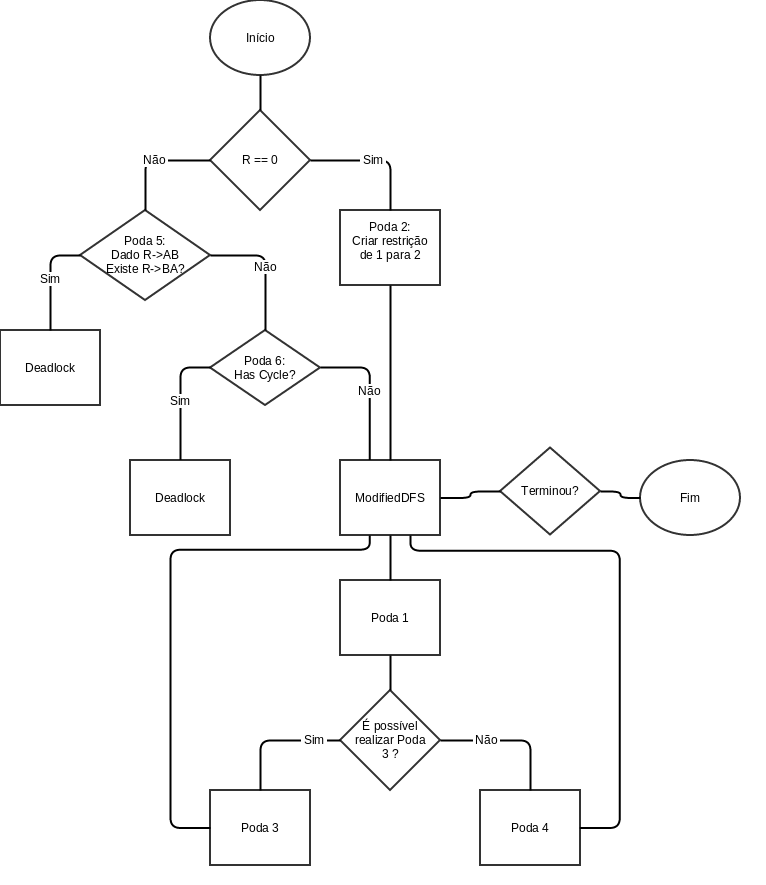
\includegraphics[scale=0.4]{tp2_podas.png}
\caption{Diagrama de podas}
\end{figure}

\section{Análise Teórica do Custo Assintótico de Tempo}
\paragraph{}

O Problema do Caixeiro Viajante, como já citado acima, possui complexidade fatorial. Para demonstrar isso, será provado abaixo que a sua versão de decisão (versão sim-não) faz parte dos chamados problemas \textbf{NP-completo}.

\subsection{Prova NP-completo para o Problema do Caixeiro Viajante}
\paragraph{}
O Problema do Caixeiro Viajante, em sua versão de decisão, pode ser descrito como: dado um grafo completo \textbf{G}(v, e) e uma constante \textbf{k}. É possível sair do primeiro vértice, percorrer todos os outros, sem repetição, e voltar ao primeiro com custo menor ou igual a \textbf{k}?
\paragraph{}
Em primeiro lugar, é necessário demonstrar que mesmo com todas as restrições, o problema ainda pode cair em um caso que necessite de de percorrer (n - 1)! caminhos, logo ainda é exponencial. Pelo Diagrama de Podas demonstrado acima, pode-se perceber que é possível que não haja restrições, logo será criada uma restrição que irá reduzir pela metade o tamanho da árvore de caminhos. Dessa maneira existem (n-1)!/2 caminhos a serem percorridos. Além disso, a solução pode ser o último caminho verificado, o que impediria as podas 1, 3 e 4, sendo esse o pior caso. Ainda seria necessário verificar (n - 1)!/2 caminhos.


\subsection{Prova NP}
\paragraph{}
Seja $C$ = \{V1, V2, ..., Vj, V1\} , uma solução para o PCV. O seguinte algoritmo verifica se $C$ é uma solução para PCV em $G$.

\begin{algorithm}
\caption{Verify TSP solution}
\begin{algorithmic}
\Function{verifySolution}{$G$, $C$, $k$, $n$}
	\State \Comment{Se C possuir menos elementos do que o número de vértices de G + 1 (A aresta que volta a V1) então é uma solução inválida.}    
    \If{$C$.numberOfElements() != $G$.numberOfVertex() + 1}
		\State \Return false;    
    \EndIf
    \State \Comment{Verifica se há repetições de vértices e se todos os vértices fazem parte do grafo}
	\State Seja $aux$ um vetor booleano
	
	\For{$i$ = 0; $i$ minor than $n$; $i$++}
		\If{!$aux$[$C$[$i$]]}		
			\State $aux$[$C$[$i$]] = true;	
		\Else
			\State \Return false;
		\EndIf    
    \EndFor
    
    \State \Comment{Verifica se o caminho é menor do que K}
    \For{$i$ = 0; $i$ minor than $n$ - 1; $i$++}
		\State $path$ += $G$[$i$][$i$ + 1];		
    \EndFor
    \State $path$ += $G$[$n$ - 1][0];
    		\If{$path$ minor or equal $k$}		
			\State \Return true;	
		\Else
			\State \Return false;
			\EndIf
\EndFunction
\end{algorithmic}
\end{algorithm}

\paragraph{}
O algoritmo acima possui complexidade linear, pois percorre os vértices do grafo 2 vezes, logo possui complexidade O(v).

\subsection{Prova NP-completo}
\paragraph{}
Para provar que PCV pertence a NP Completo, utilizarei o problema do Caminho Hamiltoniano. Que é descrito a seguir:
\paragraph{}
\textit{Dado o grafo G(v, e) e um vértice V0, é possível partir de V0, percorrer todos os vértices, sem repetição, e retornar a V0?}

\subsubsection{Transformação}
\paragraph{}
Seja G(V, E) uma instância do CH, construiremos uma instância G'(V, E') do PCV, a partir dela, da seguinte maneira: Se existe uma aresta de Va para Vb em G, então criar uma aresta Va para Vb em G' com peso 0. Caso contrário, criar uma aresta de Va para Vb com peso 1.

\subsubsection{Prova}
\paragraph{}
Seja \textit{h} uma viagem em G. Pela construção de G', ela possui custo 0 no grafo G'. Logo é uma viagem em G' com custo 0.
\paragraph{}
Por outro lado, seja \textit{m} uma viagem em G' com custo máximo 0. Tendo em vista a construção do grafo G', a única maneira de obter custo 0, é percorrer o Ciclo Hamiltoniano.
\paragraph{}
Dessa maneira, G tem um Ciclo Hamiltoniano \textbf{se e somente se} G' tem uma viagem de custo máximo 0 e G é solução para CH \textbf{se e somente se} G' é solução para G'.

\section{Análise Teórica do Custo Assintótico de Espaço}
\paragraph{}
O programa necessita de pouco espaço em memória para ser executado.
No início são alocadas duas matrizes de 23x23 para as cidades e as restrições.

\subsubsection{ModifiedDfs}
A principal função do programa, utiliza dois vetores de V posições e, como é recursiva, mantém uma pilha de recusão do tamanho de V. Sendo assim, possui custo linear O(V).

\section{Análise Experimental do Custo Assintótico}
\paragraph{}
Para verificar o custo assintótico, realizei testes utilizando entradas que caiam no pior caso, descrito na seção \textbf{3.1}. Para medi-los utilizei a função time do ubuntu.
\subsubsection{Análise Experimental}
\begin{figure}[!h]
\centering
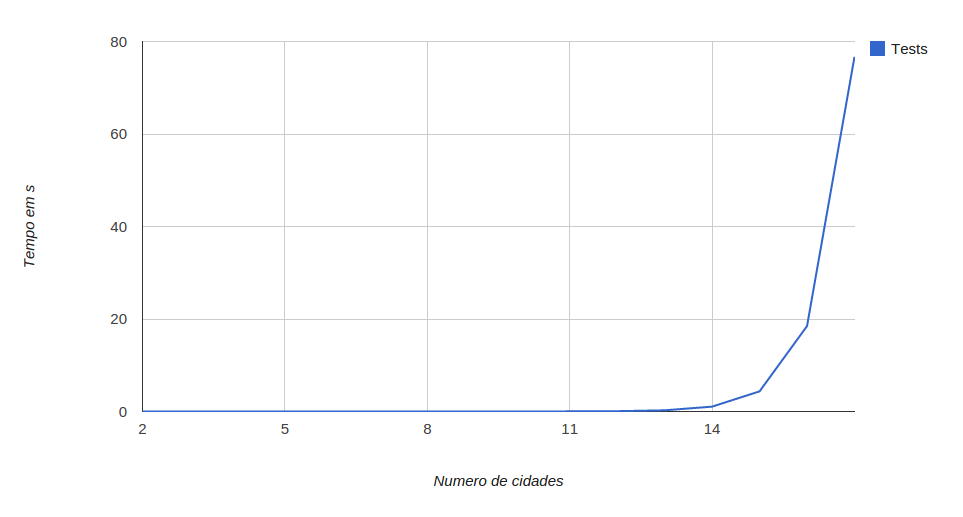
\includegraphics[scale=0.4]{analise.png}
\caption{Testes realizados}
\end{figure}


\section{Conclusão}
\paragraph{}
A execução de problemas NP-completo pode ser muito custosa devido a sua natureza exponencial. Todavia, é possível, de acordo com as características das variações do problema, criar melhorias que permitem executar diversos casos em curto tempo. 
\paragraph{}
As técnicas de Branch and Bound realizadas nesse trabalho permitiram a execução de diversas instâncias do PCV que com um simples algoritmo de força bruta são impossíveis de serem realizadas.

\end{document}
